\begin{figure}[ht] 
 	\centering 
 	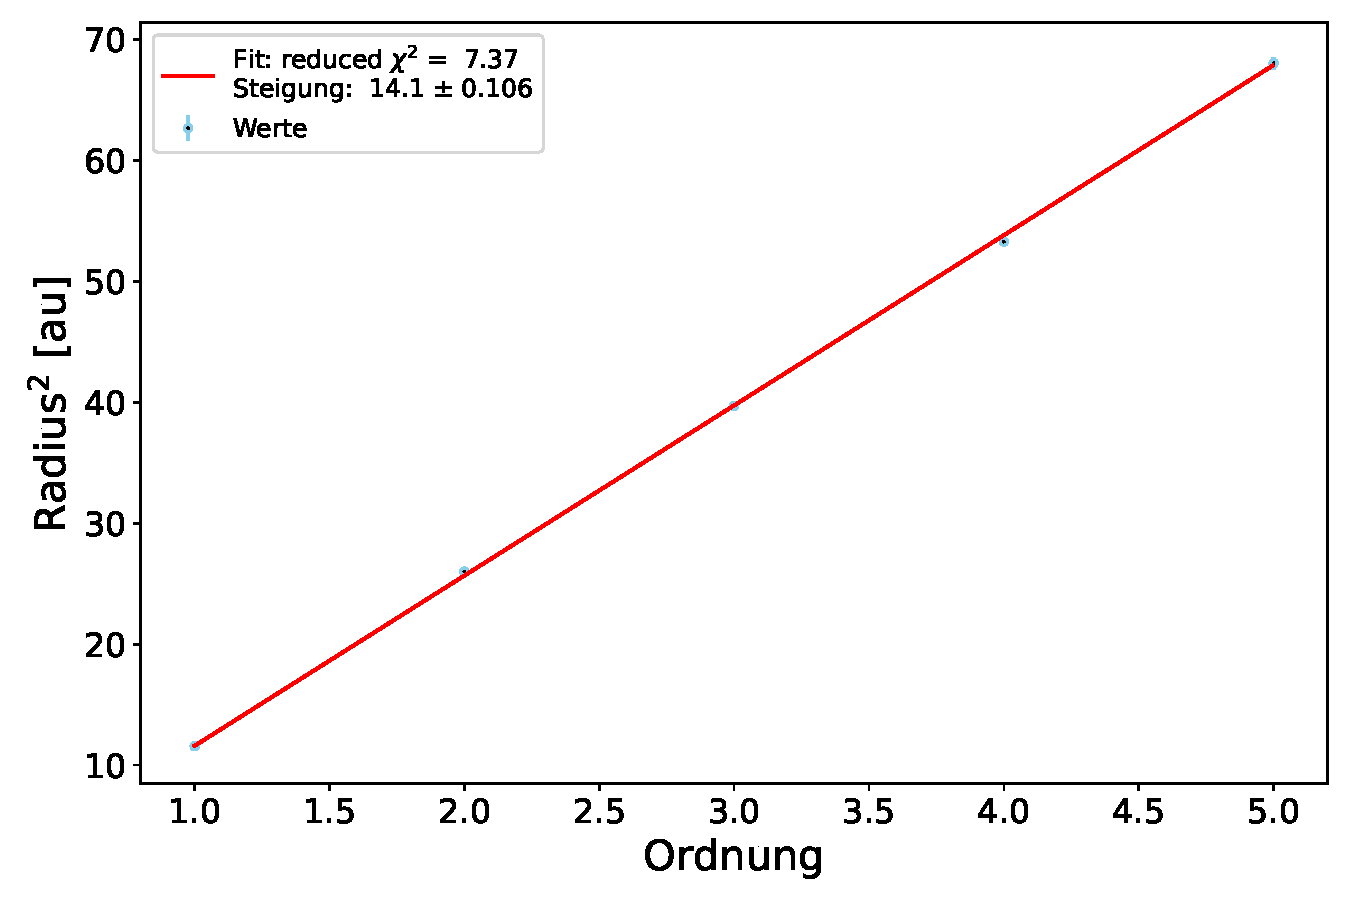
\includegraphics[width= 0.65 \textwidth]{Fits/messung2_Ring3_tim_Fit.pdf} 
	\caption{messung2_Ring3_tim, Fit} 
 	\label{fig:messung2_Ring3_tim, Fit} 
\end{figure}
 \\ 
\begin{table}[ht] 
\centering 
\caption{messung2_Ring1_tim, Fit Parameter Tabelle} 
\label{tab:my-table}
\begin{tabular}{|l|c|}
\hline
Parameter Name	&	Wert \\ \hline
slope	&	 14.074 \pm  0.106\\ \hline
intercept	&	-2.4732 \pm  0.183\\ \hline
\end{tabular} 
\end{table}